\section{Contextual features}
\label{scene}
This section describes our methodology for capturing background information or \textit{contextual features}. We present a novel approach for including description of background trajectories. We argue that combining a pure foreground description \cite{wang2013} with additional surrounding cues have a significant contribution to actions description. To obtain these background trajectories, we perform a weak foreground-background separation based on the trajectory displacement. Then, we explicitly model the global motion in the video and the context appearance using those background feature points. 


\subsection{Foreground-background segmentation}
In order to recover information related with actions context, we need separate track features as foreground or background. A lot of information related with the actor are included on the Improved Trajectories approach. It results beneficial when capturing the spatio-temporal appearance of human actions. However, we claim that modeling contextual information needs to be performed on background feature points. We apply a simple strategy to weakly labeling trajectory features. We compute trajectories as described in \cite{wang2013}, but also compute the sum of the frobenius norm for the displacement vector as follow:
\begin{equation}
D = \sum _{j=t}^{t+L-1}\left ( (x_{t+1}-x_t)^2, (y_{t+1}-y_t)^2 \right ),
\end{equation}
this measure allow us to perform a binary trajectory segmentation: (a) if $D>\alpha$ trajectory is labeled as foreground and (b) for $D<=\alpha$ correspond a background trajectory. Empirically, we set this threshold value to $\alpha=3$ pixels.


Figure \ref{fig:approach} illustrates weak trajectory segmentation results in different video sequences. Red and blue color represent feature points associated with the foreground and background features respectively. We notice that this simple approach allow us to weakly separate between the action trajectories and the background. 

\begin{figure*}[t!]
\begin{center}
%\fbox{\rule{0pt}{3in} \rule{0.9\linewidth}{0pt}}
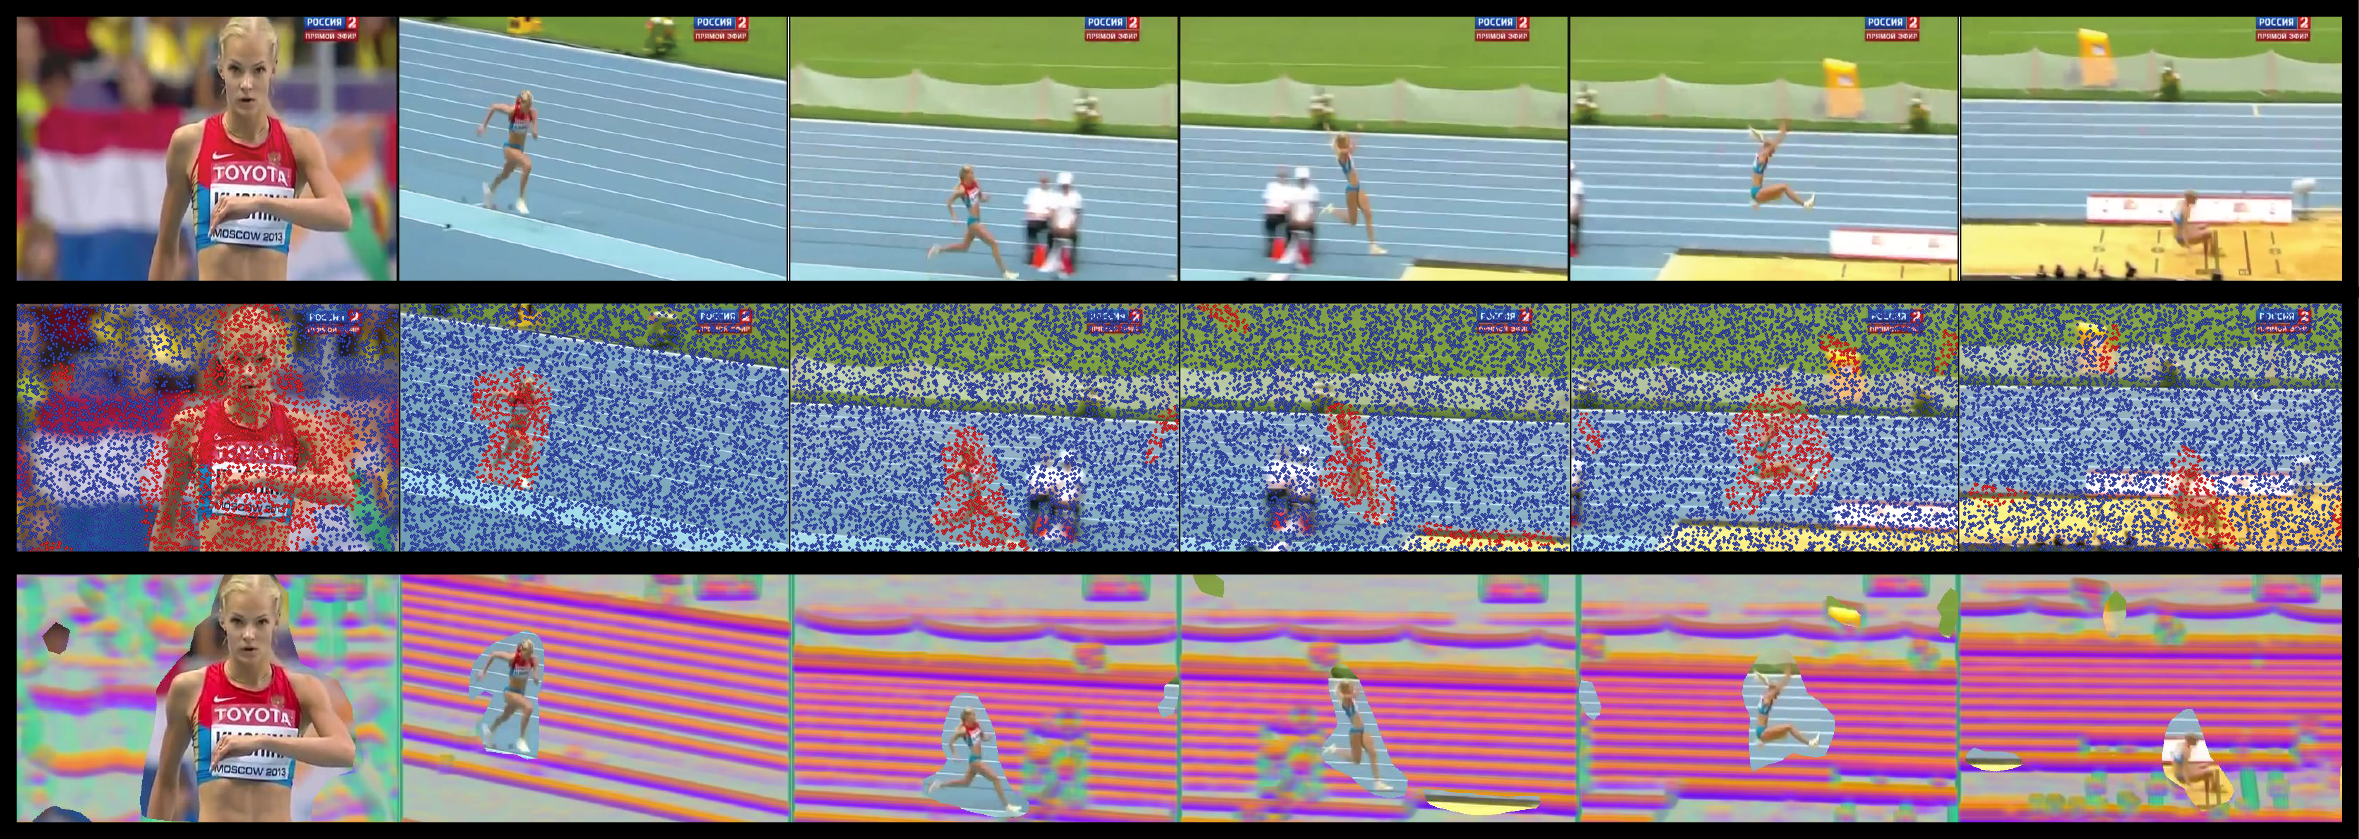
\includegraphics[width=0.98\linewidth]{fig/approach.png}
\end{center}
\caption{Illustration of weak segmentation of feature points. }
\label{fig:approach}
\end{figure*}

\subsection{Camera motion}
Since videos are normally filmed with an intention, the camera motion is a helpful component to make a better description of human actions. Recent approaches relies on canceling the camera motion in order to capture a more pure action cues. In contrast to most existing works, we employ a low level feature for capturing the global motion in the video. 
\subsection{Context appearance}
Human actions could be recognized by a set of cues. Beyond the movements, the scenario where action is executed is a critical component to recognize actions. For example, springboard can be only executed if there is a pool where submerge. It motivate us to encode visual appearance of the scene. This context appearance is encoded computing SIFT \cite{lowe2004} descriptors around the trajectory points associated with the background. We compute SIFT features in dense fashion and then we filter out those feature points that fall within our foreground mask. Context appearance focuses more on the scenario itself, as observed in Figure \ref{fig:approach}. 
